% ============================================================
% 3. DISEÑO DE LA SOLUCIÓN
% (escenario de aplicación (requisito numeral 5 del parcial:
%  diagrama + descripción breve) y arquitectura de la solución)
% ============================================================
\section{Diseño de la Solución}
\label{sec:diseno}

% ------------------------------------------------------------
% 3.1 Escenario de aplicación
% ------------------------------------------------------------
\subsection{Escenario de Aplicación}
\label{sec:escenario}

% Diagrama obligatorio del numeral 5. Fuente: docs/diagramas/escenario.puml
% (regenerar con «task diagramas»).

\begin{figure*}[!t]
  \centering
  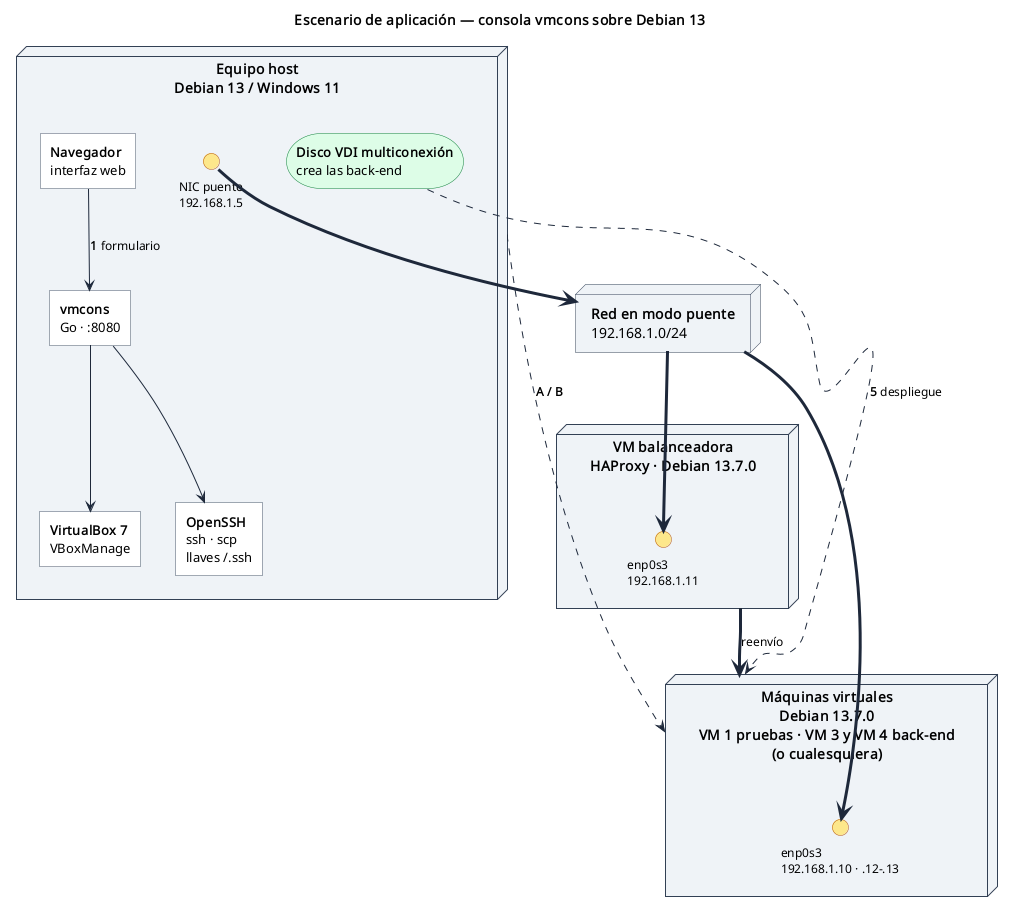
\includegraphics[width=\textwidth]{images/escenario}
  \caption{Escenario utilizado para desarrollar y probar la solución:
  equipo host, software de virtualización, máquinas virtuales con su
  sistema operativo, interfaces de red y direcciones IP, mecanismos de
  comunicación, disco de almacenamiento y flujo general de la
  automatización. El enlace A/B es el mecanismo de comunicación con la
  VM: A corresponde a las Guest Additions (solo antes de instalar SSH)
  y B al acceso por SSH con llaves (después, de forma exclusiva).}
  \label{fig:escenario}
\end{figure*}

% Flujo de proceso: se declara junto a la Figura 1 para que la
% colocación de la figura sea anterior al final de la sección.
% Fuente: docs/diagramas/flujo-procesos.puml (regenerar con «task diagramas»).
\begin{figure*}[!t]
  \centering
  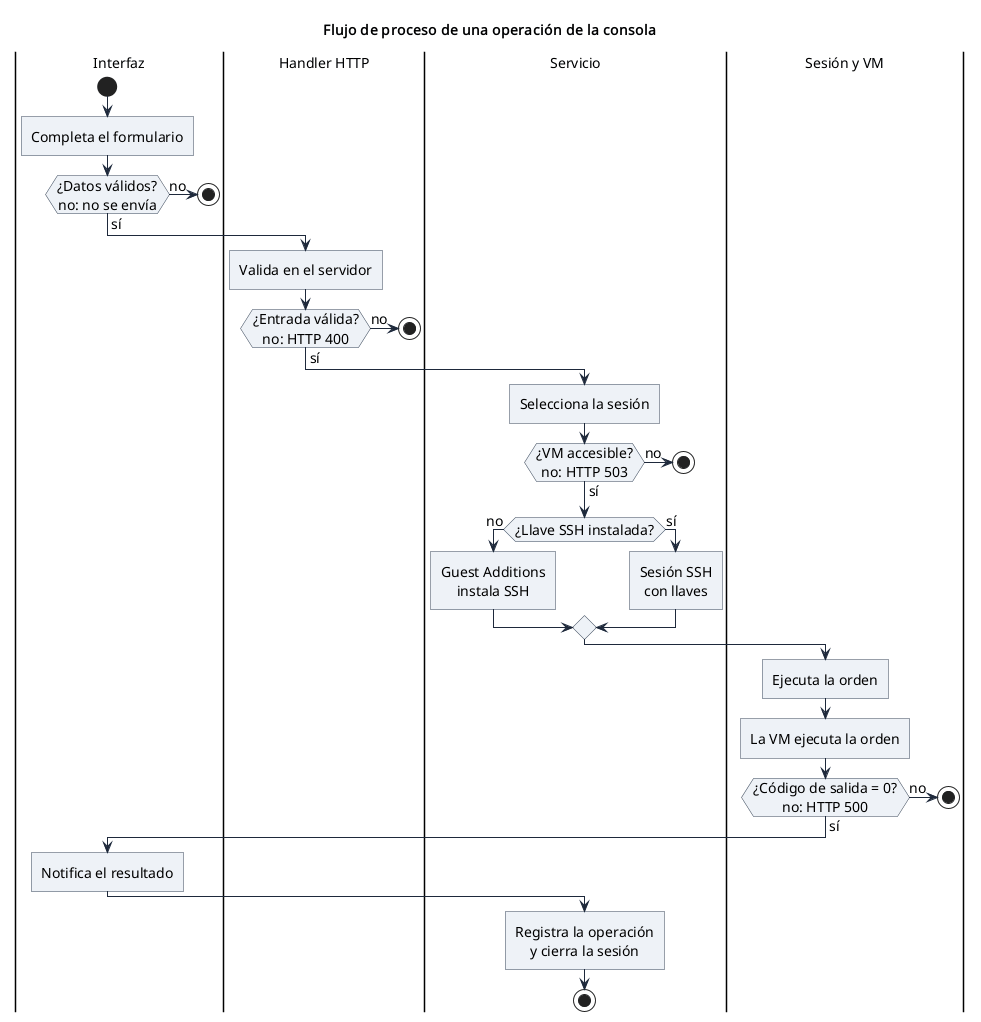
\includegraphics[width=0.95\textwidth]{images/flujo-procesos}
  \caption{Flujo de proceso de una operación solicitada desde la interfaz,
  con los responsables de cada etapa: interfaz, validación en el servidor,
  selección de sesión, ejecución no interactiva y notificación del
  resultado o del error técnico.}
  \label{fig:flujo-proceso}
\end{figure*}

\subsubsection{Descripción del Escenario}
\label{sec:desc-escenario}

La solución se desarrolla y se prueba sobre el escenario de la
\cref{fig:escenario}. El \emph{equipo host} es el equipo físico donde se
instala Oracle VM VirtualBox~7 y se ejecuta la consola \texttt{vmcons};
su sistema operativo puede ser GNU/Linux Debian~13 o Windows~11, ya que
la consola se compila como un binario único sin dependencias en tiempo de
ejecución. La consola publica la interfaz web en el puerto \texttt{8080}
y es accedida desde un navegador instalado en el mismo equipo.

La red física funciona en modo puente (bridge) sobre la subred
\texttt{192.168.1.0/24}, con un servidor DHCP/DNS en \texttt{192.168.1.1}.
La tarjeta de red del anfitrión recibe \texttt{192.168.1.5} y las
máquinas virtuales reciben direcciones de la misma subred en su
interfaz \texttt{enp0s3}: \texttt{192.168.1.10} a \texttt{192.168.1.13}.
Al estar en modo puente, las VM quedan visibles en la red local con una
dirección propia, lo que permite probar servicios de red reales como SSH
o HAProxy sin reglas de reenvío de puertos.

Todas las máquinas virtuales ejecutan GNU/Linux Debian~13.7.0. El
balanceador ocupa un nodo propio en la \cref{fig:escenario} porque es la
máquina del módulo de HAProxy: recibe las peticiones en
\texttt{192.168.1.11} y las reenvía, a través de la misma red, a los
servidores del back-end. Las restantes se resumen en un único contenedor
etiquetado como «o cualesquiera»: la VM~1 es la máquina de pruebas sobre
la que se ejecutan los módulos de preparación del sistema, gestión de
usuarios y servicios con systemd, y la VM~3 y la VM~4 son los servidores
del back-end; la consola abre sesión con la máquina que corresponda en
cada operación, de modo que el conjunto de VM cambia según las pruebas.
Estas últimas se crean a partir de un \emph{disco virtual VDI
de multiconexión} (multiattach) con carga diferencial guardado en el
anfitrión, de modo que cada back-end arranca desde la misma imagen base
sin duplicar el disco y puede añadirse o eliminarse una máquina más
utilizando el mismo archivo.

\subsubsection{Mecanismo de Comunicación}
\label{sec:mecanismo-com}

La consola se comunica con la máquina virtual mediante dos mecanismos,
marcados como \textbf{A} y \textbf{B} en la \cref{fig:escenario}.

El \textbf{mecanismo A} se basa en las Guest Additions
\parencite{guestadditions} y se usa \emph{únicamente antes} de instalar
SSH. La consola obtiene la dirección IP de la VM con
\texttt{VBoxManage guestproperty get} sobre la propiedad
\texttt{/VirtualBox/GuestInfo/Net/0/V4/IP}, genera el par de llaves en el
anfitrión, instala \texttt{openssh-server}, copia la llave pública al
archivo \texttt{authorized\_keys} del usuario \texttt{root} y deshabilita
el acceso por contraseña. Las órdenes se ejecutan con
\texttt{VBoxManage guestcontrol run} y los archivos se transfieren con
\texttt{guestcontrol copyto}.

El \textbf{mecanismo B} es el acceso por SSH con llaves de autenticación
\parencite{rfc4252}, mediante el cliente OpenSSH del anfitrión
(\texttt{ssh} y \texttt{scp}). Una vez instalado SSH, \emph{toda} la
comunicación posterior entre la consola y la máquina se realiza por este
canal, tal como exige el enunciado: el mecanismo A deja de utilizarse y
la consola trabaja de forma exclusiva sobre SSH, con la llave privada
resguardada en el equipo anfitrión.

\subsubsection{Flujo General de la Automatización}
\label{sec:flujo-escenario}

Todo módulo de la consola recorre el mismo flujo: (1) el usuario completa
el formulario en el navegador y lo envía; (2) la consola valida los datos
y selecciona la sesión adecuada, es decir, decide si aún necesita Guest
Additions o si ya puede trabajar por SSH; (3) ejecuta la orden de forma
no interactiva sobre la máquina virtual; (4) la máquina devuelve la
salida y la consola notifica el resultado, o bien presenta un mensaje de
error comprensible junto con la información técnica de diagnóstico; y (5)
el disco multiconexión permite ampliar el escenario creando nuevas
back-end para las pruebas de balanceo de carga.

% ------------------------------------------------------------
% 3.2 Arquitectura de la solución
% ------------------------------------------------------------
\subsection{Arquitectura de la Solución}
\label{sec:arquitectura}

\subsubsection{Visión General de la Aplicación}
\label{sec:vision-general}

La consola es una aplicación web escrita en Go que se sirve con el
paquete estándar \texttt{net/http}. La interfaz está organizada por
módulos ---preparación del sistema, gestión de usuarios, servicios con
systemd y balanceo de carga---, y cada módulo presenta un formulario con
los campos y las casillas de verificación que la operación requiere.

Toda operación sigue el ciclo de la \cref{fig:flujo-proceso}: validación
en el cliente para dar respuesta inmediata, validación en el servidor
sobre los parámetros crudos (que es la que realmente decide), selección
de la sesión, ejecución no interactiva de la orden y notificación del
resultado. Si la validación falla, la operación \emph{no} llega a la
máquina virtual y la respuesta indica el campo y el motivo; si la orden
se ejecuta y termina con un código de salida distinto de cero, la
respuesta conserva la orden ejecutada, el código de salida y la salida de
error estándar para que el usuario pueda diagnosticar el problema. Las
respuestas son documentos JSON con un campo \texttt{ok}, un
\texttt{mensaje} comprensible y, cuando falla, los campos
\texttt{operacion} y \texttt{tecnico} con el detalle técnico.

\subsubsection{Estructura del Proyecto}
\label{sec:estructura-proyecto}

El proyecto se organiza en capas para que el núcleo de la aplicación no
dependa de VirtualBox, de las Guest Additions ni de OpenSSH:

\begin{itemize}
  \item \texttt{main.go}: único punto de composición. Aquí se
  instancian los adaptadores y se inyectan a los servicios y a los
  manejadores HTTP.
  \item \texttt{internal/core/domain}: tipos del dominio
  (\texttt{Command}, \texttt{Result}, \texttt{Target},
  \texttt{MachineState} y \texttt{ExitError}) sin dependencias externas.
  \item \texttt{internal/core/ports}: interfaces \texttt{Executor},
  \texttt{Machine}, \texttt{Connector} y \texttt{Session} que expresan lo
  que la aplicación necesita del exterior.
  \item \texttt{internal/adapters}: las implementaciones concretas
  \texttt{localproc} (procesos del sistema operativo anfitrión),
  \texttt{vbox} (VirtualBox y Guest Additions) y \texttt{ssh} (cliente
  OpenSSH).
  \item \texttt{internal/services}: los casos de uso de cada módulo;
  dependen solo de los puertos del núcleo.
  \item \texttt{internal/handlers}: enrutan las peticiones HTTP y
  validan las entradas; no contienen lógica de negocio.
  \item \texttt{web}: los módulos HTML y los archivos estáticos de la
  interfaz.
\end{itemize}

Los adaptadores traducen su vocabulario al dominio: por ejemplo,
\texttt{vbox} convierte el estado \texttt{poweroff} de VirtualBox en
\texttt{domain.MachinePoweredOff}, de modo que el núcleo nunca necesita
saber qué tecnología se está utilizando. La regla de dependencia es
simple: el núcleo no importa adaptadores, los adaptadores importan el
núcleo y la composición ocurre únicamente en \texttt{main.go}.

\subsubsection{Decisiones Tomadas Durante el Desarrollo}
\label{sec:decisiones}

Las decisiones principales del diseño son las siguientes.

\emph{Binarios del sistema, no librerías nativas.} El SDK de VirtualBox
exige COM en Windows y bindings específicos en GNU/Linux; en su lugar se
invoca \texttt{VBoxManage}, oficial y multiplataforma, y para SSH se usa
el cliente incluido en el sistema en lugar de una implementación en Go
\parencite{donovan}.

\emph{Errores tipados.} Las órdenes que terminan con un código distinto
de cero producen un \texttt{domain.ExitError} que conserva el código, la
salida estándar y la salida de error; el núcleo lo entiende sin importar
qué adaptador lo originó.

\emph{Validación antes de ejecutar y en el servidor.} Las direcciones se
modelan con \texttt{net/netip.Addr}, los nombres de usuario y de host se
comprueban con expresiones regulares y ninguna entrada cruda llega a la
máquina virtual.

\emph{Un solo flujo para los siete módulos.} Todos comparten el ciclo
entrada, validación, sesión, ejecución, clasificación y notificación, lo
que uniformiza los mensajes de error y hace que las pruebas sean
repetibles.

\emph{Calidad de código verificable.} El flujo de trabajo exige
formateo con \texttt{gofumpt}, análisis con \texttt{golangci-lint} y
pruebas con detector de condiciones de carrera antes de cada commit.

\FloatBarrier
